\subsection{Спектральные классы звёзд}
\begin{table}[h!]
\centering
\footnotesize
\renewcommand{\arraystretch}{1.4}
\renewcommand{\tabcolsep}{0pt}
\begin{tabularx}{\tw}{|C{0.1}|C{0.3}|C{0.23}|C{0.13}|C{0.13}|C{0.13}|}
\hline
{\bfseries Класс} & {$\mathbf{T}$, К} & {\bfseries Цвет} & {$\mathbf{M}$, $M_{\odot}$} & {$\mathbf{R}$, $R_{\odot}$} & {$\mathbf{L}$, $L_{\odot}$}\\
\hline
O & $3 \times 10^4$ --- $6 \times 10^4$ & Голубой & 60 & 15 & $1.4 \times 10^6$\\

B & $1 \times 10^4$ --- $3 \times 10^4$ & Бело-голубой & 18 & 7 & $2 \times 10^4$\\

A & $7.5 \times 10^3$ --- $1 \times 10^4$ & Белый & 3.1 & 2.1 & 80\\

F & $6 \times 10^3$ --- $7.5 \times 10^3$ & Жёлто-белый & 1.7 & 1.3 & 6\\

G & $5 \times 10^3$ --- $6 \times 10^3$ & Жёлтый & 1.1 & 1.1 & 1.2\\

K & $3.5 \times 10^3$ --- $5 \times 10^3$ & Оранжевый & 0.8 & 0.9 & 0.4\\

M & $2 \times 10^3$ --- $3.5 \times 10^3$ & Красный & 0.3 & 0.4 & 0.04\\
\hline
\end{tabularx}
\caption{Современная спектральная классификация звёзд}
\end{table}

Помимо основных спектральных классов звёзд существуют и дополнительные:
\begin{enumerate}[1)]
\item Класс W --- звёзды Вольфа-Райе, очень тяжёлые яркие звёзды с температурой порядка $70000$~К и интенсивными эмиссиоными линиями спектра.
\item Класс L --- звёзды или коричневые карлики с температурой $1500 - 2000$~К и соединениями металлов в атмосфере.
\item Класс T --- метановые коричневые карлики с температурой $700 - 1500$~К.
\item Класс Y ---  очень холодные (метано-аммиачные) коричневые карлики с температурой ниже $700$~К.
\item Класс C --- углеродные звёзды, гиганты с повышенным содержанием углерода. Ранее относились к классам R и N.
\end{enumerate}

Мнемонические правила для запоминания спектральных классов:
\begin{enumerate}[1)]
\item\textbf{O}h \textbf{B}e \textbf{A} \textbf{F}ine \textbf{G}irl, \textbf{K}iss \textbf{M}e \textbf{R}ight \textbf{N}ow \textbf{S}weetheart.
\item\textbf{W}ell, \textbf{O}nce \textbf{B}ritish \textbf{A}stronomer has \textbf{F}ound \textbf{G}alaxy, \textbf{K}new \textbf{M}ass, \textbf{L}ength, \textbf{T}erm.
\item Вообразите: \textbf{О}дин \textbf{Б}ритый \textbf{А}нгличанин \textbf{Ф}иники \textbf{Ж}евал \textbf{К}ак \textbf{М}орковь --- \textbf{Р}азве \textbf{Н}е \textbf{С}мешно?
\end{enumerate}

\term{Диаграмма Герцшпрунга-Рассела} показывает зависимость между светимостью, спектральным классом и температурой поверхности звезды. 

\begin{figure}
	\centering
%	\begin{tikzpicture}
% 		\begin{axis}[
% 						height	=	12cm,
% 						width	=	10cm,
% 						ymax	=	15.,
% 						ymin	=	-10.,
% 						y dir	=	reverse,
% 						xmax	=	2.,
% 						xmin	=	-.5,
% 						axis x line* = bottom,
% 						axis y line* = right,
% 						xlabel=$B-V$,
% 						y label style = {at={(axis description cs: 1.2, 0.5)}, rotate=180}, 
% 						ylabel	=	{Абсолютная звёздная величина $M$, $~^m$}
% 					]
%%			\addplot+[only marks, mark = o, mark options={scale=0.2, black}] table[x=f, y=m]{data/light-curve-D-Cep.txt};
% 		\end{axis}
% 		\begin{semilogyaxis}[	
% 						height	=	12cm,
% 						width	=	10cm,
% 						ymax	=	8.312e5,
% 						ymin	=	8.312e-5,
% 						xmax	=	2.,
% 						xmin	=	-.5,
% 						minor x tick num = 0,
% 						minor y tick num = 01,
% 						xtick = {-0.264, 0, 0.3, 0.58, 0.791, 1.57},
% 						xticklabels = {B0, A0, F0, G0, K0, M0},
% 						axis x line* = top,
% 						axis y line* = left,
% 						xlabel	=	{Спектральный класс}, 
% 						x label style = {at={(axis description cs: 0.5, 1.11)}, rotate=0},
% 						ylabel	=	{Светимость $L$, $L_\odot$},
% 						ymajorgrids	 =	false,
% 						xmajorgrids	 =	false	
%    				]
%		\end{semilogyaxis}
% 	\end{tikzpicture}
	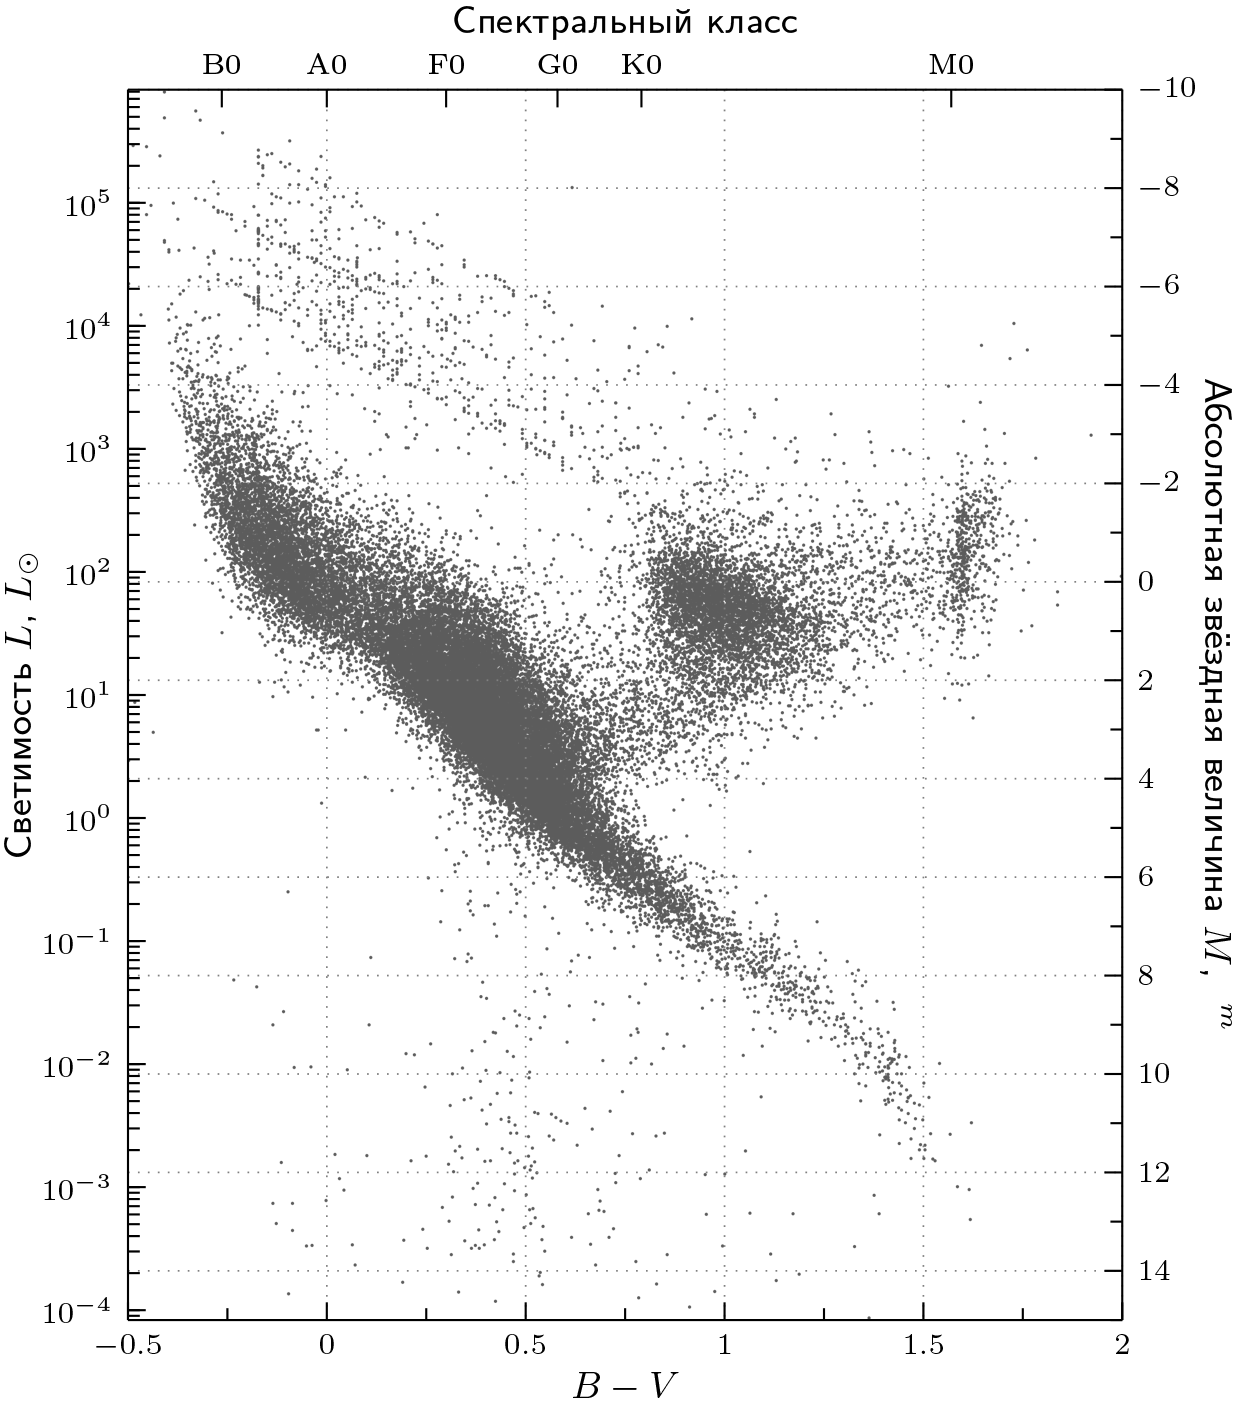
\includegraphics[width=10cm]{gr}
 	\caption{Диаграмма Герцшпрунга--Рассела}
 	\label{pic:d-cep}
\end{figure}


Была предложена примерно в 1910 году независимо Эйнаром Герцшпрунгом и Генри Расселом. Диаграмма используется для классификации звёзд и соответствует современным представлениям о звёздной эволюции.

Около $90 \%$ звёзд находятся на главной последовательности. Их светимость обусловлена термоядерными реакциями превращения водорода в гелий. Выделяется также несколько ветвей проэволюционировавших звёзд --- гигантов, в которых происходит горение гелия и более тяжёлых элементов. В левой нижней части диаграммы находятся полностью проэволюционировавшие белые карлики.

